% \strut \vspace{35pt} %\vspace{40pt}
\strut \vspace{20pt} %\vspace{40pt}

\Huge{\textsc{Astronomy as a Field:}}\\ 
\Large{\textsc{A Guide for Aspiring Astrophysicists}}\\
\\
\Large{SIRIUS B}\\
\large{\href{https://siriusb.org}{siriusb.org}}

% \vspace{70pt}
\vspace{40pt}
\Large{\emph{Organizer}}\\
\vspace{-10pt}
\normalsize

\begin{wrapfigure}{l}{0.2\textwidth}
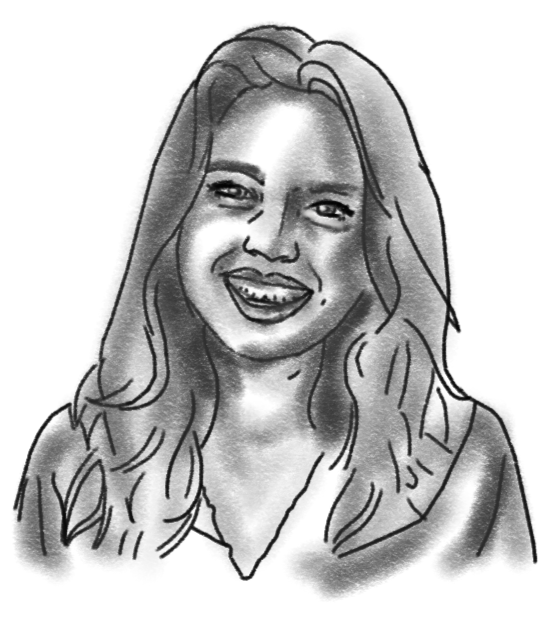
\includegraphics[width=0.9\linewidth]{portraits/ava_again.png}
\end{wrapfigure}
\textbf{Ava Polzin} is a PhD candidate in Astronomy \& Astrophysics at the University of Chicago. Her work focuses on understanding star formation and the baryon cycle in the smallest dwarf galaxies. She lives in Chicago's Hyde Park neighborhood with her two cats, Emma (a mercurial calico) and F\'{e}licette (named for the first cat in space; see last page for the story of the \textit{original} F\'{e}licette). The mini-grant she received from the International Astronomical Union's North American Regional Office of Astronomy for Development and the Heising-Simons Foundation for this work went a long way in printing these booklets thanks to the contributions of more than thirty (!!) women, who are committed to encouraging girls in their pursuit of astrophysics. This effort is the culmination of years of Ava's work toward making science more equitable and accessible (see \href{https://siriusb.org}{siriusb.org} for recent details) and in addition to writing all of the uncredited sections (and some of the credited ones), she will be running the synchronous VERGE program, for which this guide was created, in January 2024 with some of the women who contributed here also giving talks/presentations to the participating girls.

The printing of this work for the 2024 VERGE program is funded by the IAU NA-ROAD and the Heising-Simons Foundation under the Women and Girls in Astronomy Program.
\\

\vfill
\begin{center}
\textit{\small All art by Julie Malewicz.}  
\end{center}

\pagebreak
\LARGE{\emph{Contributors (Listed Alphabetically)}}
\normalsize
\vspace{20pt}

\Large{\emph{Section Authors}}\\
\vspace{-10pt}
\normalsize

\begin{wrapfigure}[5]{l}{0.22\textwidth}
\vspace{-\intextsep}
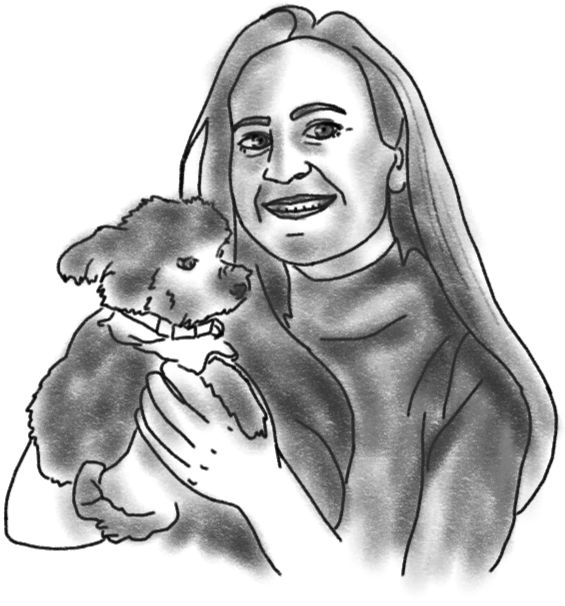
\includegraphics[width=0.9\linewidth]{portraits/yasmeen.png}
\end{wrapfigure}
\textbf{Yasmeen Asali} is a PhD candidate in Astronomy at Yale University. She works on understanding how star formation evolves in low mass galaxies and how a galaxy’s environment can impact this evolution. She is interested in the intersection of data science and astronomy, and passionate about teaching.\\
\\


\begin{wrapfigure}[4]{r}{0.22\textwidth}
\vspace{-2.5\intextsep}
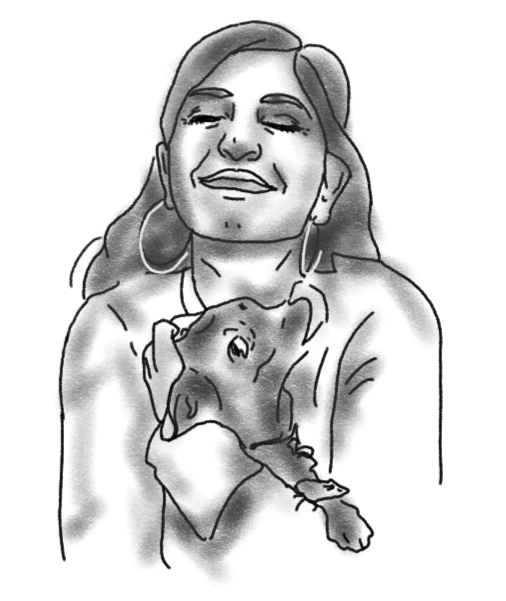
\includegraphics[width=0.9\linewidth]{portraits/sanah.png}
\end{wrapfigure}
\textbf{Sanah Bhimani} is a PhD candidate in physics at Yale University. She works on CMB experiments like the Simons Observatory. Sanah and her rescue dog Etta enjoy walking around New Haven's East Rock neighborhood.\\
\\

\begin{wrapfigure}{l}{0.22\textwidth}
\vspace{-\intextsep}
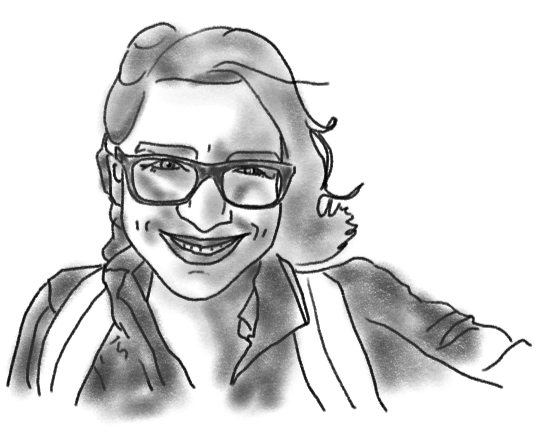
\includegraphics[width=0.9\linewidth]{portraits/madison.png}
\end{wrapfigure}
\textbf{Madison Brady} is a PhD candidate in Astronomy \& Astrophysics at the University of Chicago.  She uses high-precision spectroscopic data to measure the masses of nearby exoplanets.  She is interested in studying how rocky, Earth-like planets form and evolve around small stars.  She also wants to figure out whether or not water worlds exist.\\
\\

\begin{wrapfigure}[6]{r}{0.22\textwidth}
% \vspace{-\intextsep}
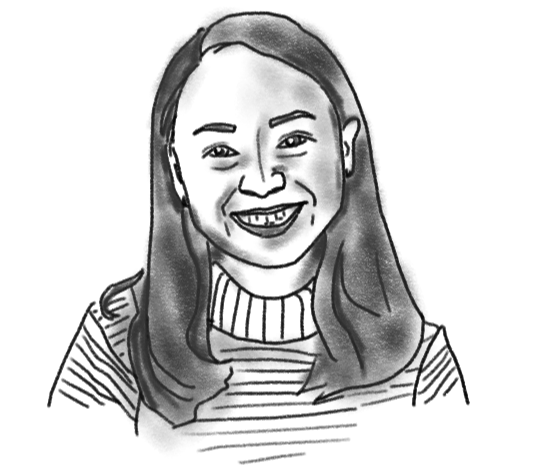
\includegraphics[width=0.9\linewidth]{portraits/mandy.png}
\end{wrapfigure}
\textbf{Mandy Chen} is a PhD candidate in Astronomy \& Astrophysics at the University of Chicago. She uses integral-unit spectroscopic data to discover and model the motions of diffuse gas surrounding galaxies.  The overarching goal of her research is to understand the interplay between galaxies and their low-density gaseous environments, and how these interactions evolve over cosmic time.\\
\\

\begin{wrapfigure}[9]{l}{0.22\textwidth}

\includegraphics[width=0.9\linewidth]{portraits/lindsay.png}
\end{wrapfigure}
\textbf{Lindsay DeMarchi} is a stellar mortician and space environmentalist. She earned her Ph.D. in Astronomy at Northwestern University by researching multi-messenger, multi-wavelength approaches to dead and dying stars. Her greatest dream is to protect and steward darkness and silence, so she volunteers with the IAU CPS, DarkSky International, and AAS. Her favorite hobby is collaborating with indie filmmakers and video game developers to make their space visions real. \\
\\

% \pagebreak

\begin{wrapfigure}[5]{r}{0.22\textwidth}
\vspace{-1.5\intextsep}
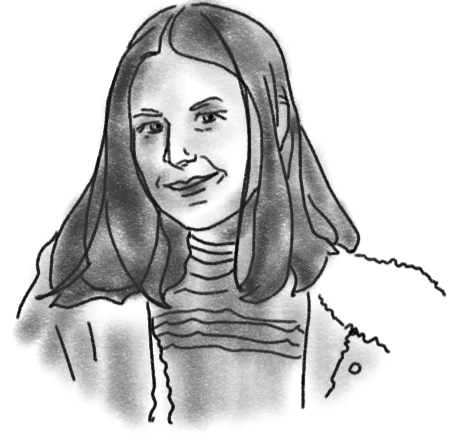
\includegraphics[width=0.9\linewidth]{portraits/michelle.png}
\end{wrapfigure}
\textbf{Michelle Gurevich} is a PhD candidate in the Theoretical Particle Physics and Cosmology group at King's College London. Her background is in general relativity and gravitational waves. She currently studies the ringdown of binary black hole mergers to test theories of gravity.\\
\\

\vspace{-10pt}

\begin{wrapfigure}[11]{l}{0.22\textwidth}
% \vspace{-\intextsep}
\vspace{20pt}
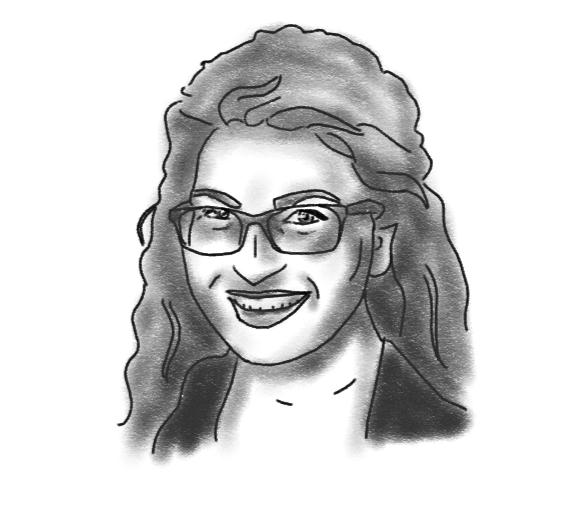
\includegraphics[width=0.9\linewidth]{portraits/emily_l.png}
\end{wrapfigure}
\textbf{Emily Lichko} is a postdoc at the University of Chicago. She received her B.S. in Physics and Applied Mathematics from the University of Michigan in 2013 and her PhD in 2020 from the University of Wisconsin - Madison, working under the supervision of Professor Jan Egedal. Her research focuses on kinetic plasma physics processes in space and astrophysical plasmas, in particular as they relate to questions of particle heating and nonlinear processes that affect the evolution of collisionless, anisotropic plasmas. Outside of her research, she enjoys swimming, biking, running, and failing to replicate recipes from the Great British Bake Off. \\
\\

\vspace{-20pt}

\begin{wrapfigure}[7]{r}{0.22\textwidth}
\vspace{-\intextsep}
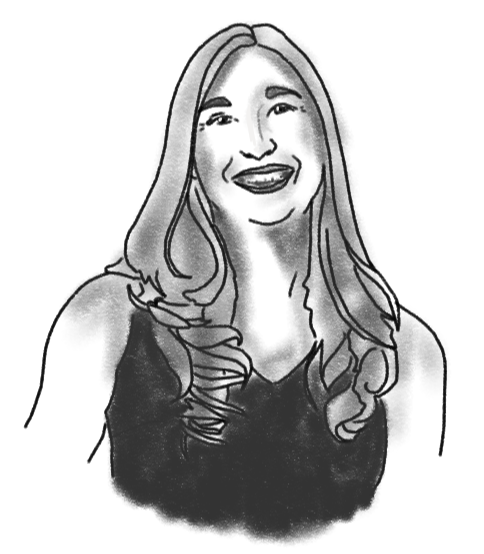
\includegraphics[width=0.9\linewidth]{portraits/emma.png}
\end{wrapfigure}
\textbf{Emma Louden} is a PhD candidate at Yale University in New Haven. She studies the geometry of exoplanetary systems. Emma is passionate about a future-focused strategy for astrophysics, engaging the public with space exploration, and applying evidence-based solutions to solve the world’s most pressing problems. She is a 2018 Brooke Owens Fellow and a 2023 Quad Fellow.
\\
\\

% \vspace{50pt}
\strut \vspace{-50pt}

\begin{wrapfigure}[7]{l}{0.22\textwidth}
% \vspace{-\intextsep}
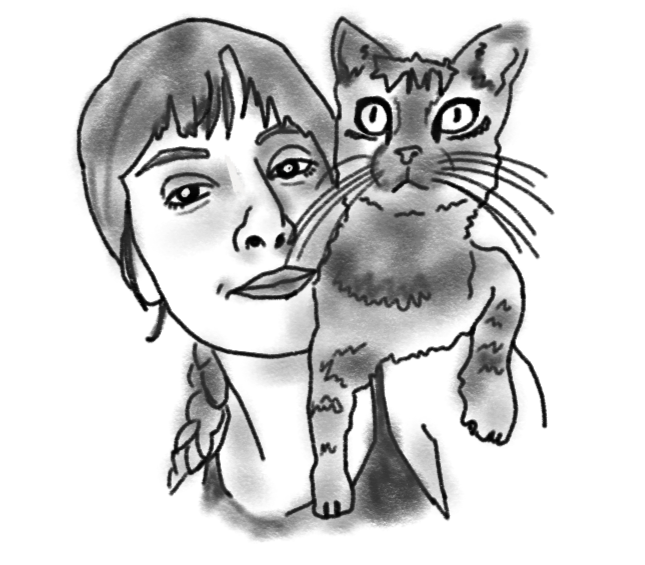
\includegraphics[width=0.9\linewidth]{portraits/julie_and_bug.png}
\end{wrapfigure}
\textbf{Julie Malewicz}  is a PhD candidate down at the Georgia Institute of Technology in Atlanta, where she's working on predicting the X-ray signal from accreting supermassive black hole binaries. She is passionate about public transit, community gardens, taking in stray cats (incl. one very persistent tabby called Ladybug) and advocating for science as a field to be more inclusive and accessible. \\
\\

\begin{wrapfigure}[3]{r}{0.22\textwidth}
\vspace{-2.5\intextsep}
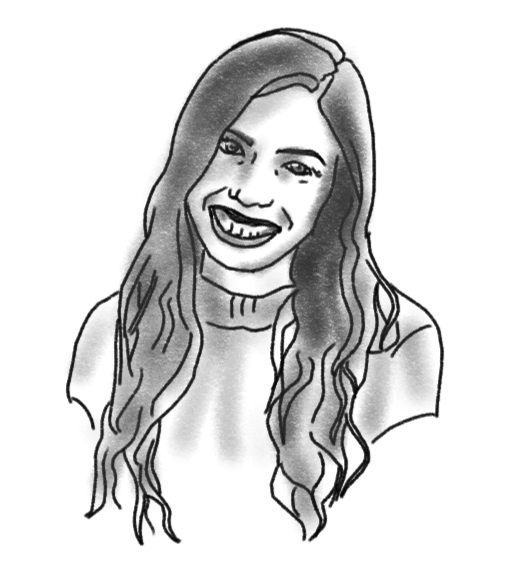
\includegraphics[width=0.9\linewidth]{portraits/samantha.png}
\end{wrapfigure}
\textbf{Samantha Pagan} is a physics Ph.D. candidate at Yale University. She researches dark matter and neutrinos to explore questions such as why our universe is made of matter.\\
\\

\begin{wrapfigure}[6]{l}{0.22\textwidth}
\vspace{-\intextsep}
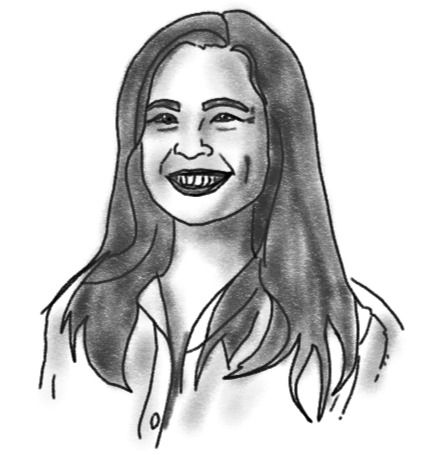
\includegraphics[width=0.9\linewidth]{portraits/malena.png}
\end{wrapfigure}
\textbf{Malena Rice} is an Assistant Professor of Astronomy at Yale University. Her research focuses on understanding the diversity of planetary systems, drawing together insights from both exoplanet systems and the solar system. Her recent work has focused on characterizing exoplanet orbital architectures and the distant solar system. \\
\\

\begin{wrapfigure}[4]{r}{0.22\textwidth}
\vspace{-1.75\intextsep}
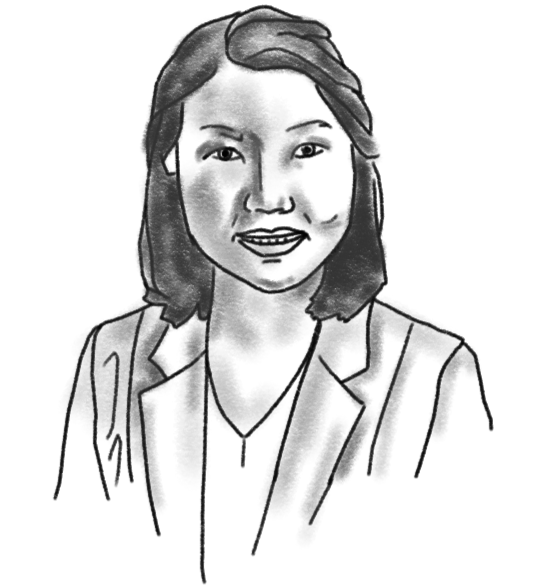
\includegraphics[width=0.9\linewidth]{portraits/zili.png}
\end{wrapfigure}
\textbf{Zili Shen} is a PhD candidate in the Yale University Department of Astronomy. She uses the Keck Observatory and the Hubble Space Telescope to observe faint galaxies. She works on discovering the biggest and most diffuse galaxies in our cosmic neighborhood.\\
\\

\begin{wrapfigure}[6]{l}{0.22\textwidth}
\vspace{-0.5\intextsep}
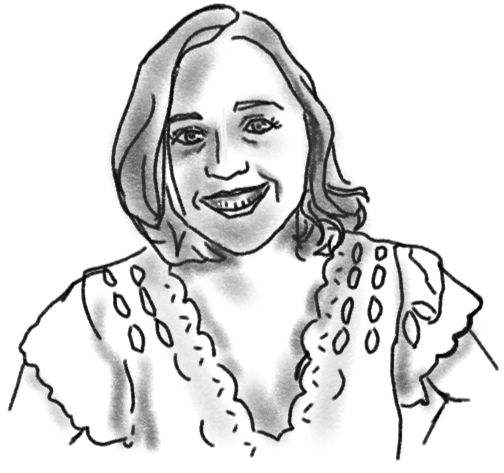
\includegraphics[width=0.9\linewidth]{portraits/emily.png}
\end{wrapfigure}
\textbf{Emily Simon} is a PhD candidate in Astronomy \& Astrophysics at the University of Chicago. She is interested in astroparticle physics and hopes to understand the origins and acceleration mechanisms for high energy particles like cosmic rays and neutrinos which likely come from the most extreme environments in the universe like supernova explosions and black hole accretion disks.\\
\\

\begin{wrapfigure}[5]{r}{0.22\textwidth}
\vspace{-1.2\intextsep}
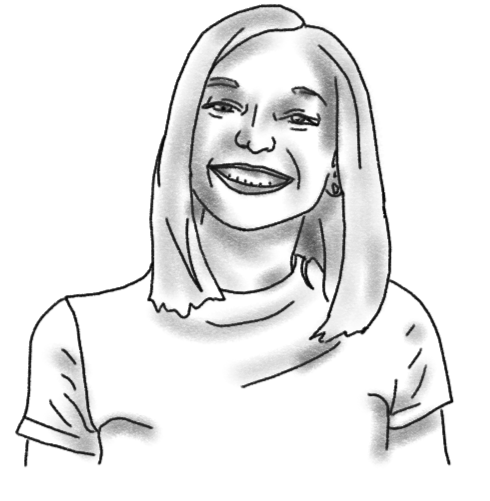
\includegraphics[width=0.9\linewidth]{portraits/candice.png}
\end{wrapfigure}
\textbf{Candice Stauffer} received her Ph.D. in Astrophysics from Northwestern University in 2023. She is an expert in using computational and machine learning methods to study stellar explosions, like supernovae, and the multi-wavelength Universe. She currently works as a Data Scientist for the City of Chicago. \\
\\

\begin{wrapfigure}[9]{l}{0.22\textwidth}
% \vspace{-\intextsep}
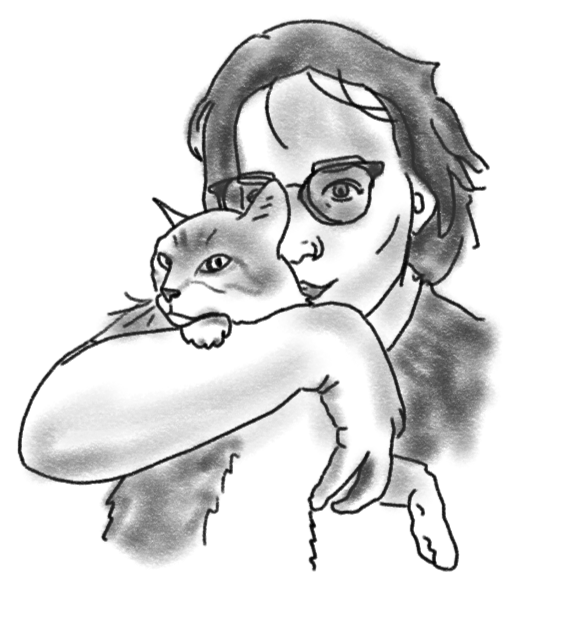
\includegraphics[width=0.9\linewidth]{portraits/luna.png}
\end{wrapfigure}
\textbf{Luna Zagorac} is a postdoctoral fellow at the Perimeter Institute for Theoretical Physics in Ontario, Canada. She is a cosmologist through and through: passionate not just about what our silly little Universe is up to, but also about all the ways we as humans interact with it and understand it. When not thinking about dark matter, inflation, and other parts of our invisible Universe, she is using data science to understand astronomical and observational practices in ancient Egypt, roller skating, reading, or playing video games. \\

% \vspace{20pt}
\pagebreak
\Large{\emph{Advice for Students}}\\
\vspace{-10pt}
\normalsize

\begin{wrapfigure}[18]{r}{0.22\textwidth}
% \vspace{-\intextsep}
\vspace{50pt}
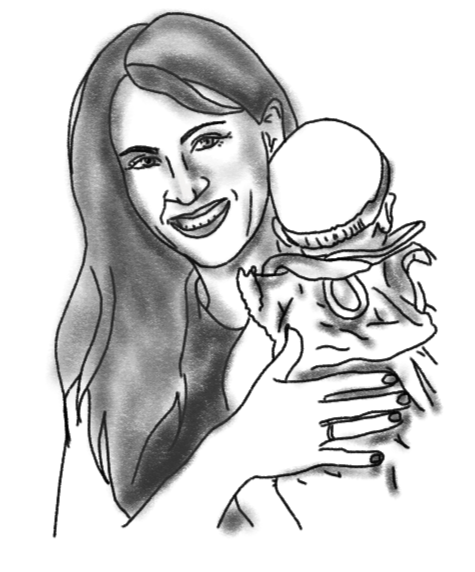
\includegraphics[width=0.9\linewidth]{portraits/katie_a.png}
\end{wrapfigure}
\textbf{Katie Auchettl} is an observational astrophysicist whose research focuses on understanding the physical processes and observational signatures of the extreme death of stars using instruments that observe across the entire electromagnetic spectrum.  Growing up in Melbourne, Australia she was lucky enough to have access to some of the darkest skies anywhere in the world. This naturally led to her excitement about studying the stars in any way she could. As a first generation university student who attended a local public school, it wasn't until university that she realised she could pursue a degree in astronomy. After finishing a PhD at Monash University in Melbourne in 2015, she was a CCAPP Postdoctoral Fellow at the Ohio State University and then an Assistant Professor at the University of Copenhagen before joining the University of Melbourne in 2020, where she is currently an Associate Professor. Apart from studying the stars, Katie is passionate about issues related to diversity, equity and inclusion in the sciences as well as outreach that allows all members of the community to be engaged in science.\\
\\

% \pagebreak

\begin{wrapfigure}[11]{l}{0.22\textwidth}
\vspace{25pt}
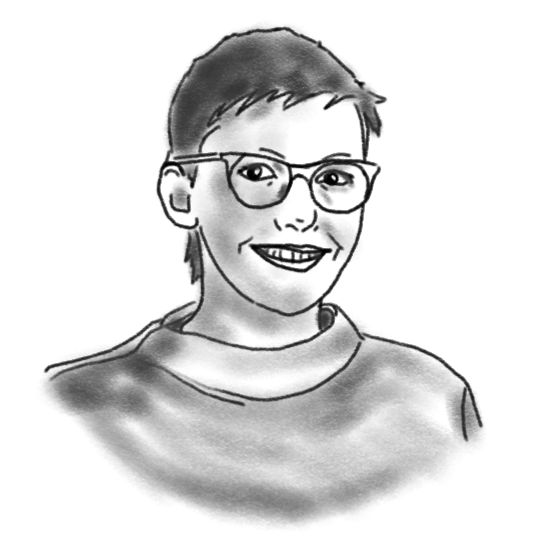
\includegraphics[width=0.9\linewidth]{portraits/katie.png}
\end{wrapfigure}
\textbf{Katie Breivik} grew up under the stars of northern Utah and southern Idaho where her family spent almost every weekend building a cabin. During the weekdays, she'd drag her parents across grocery store parking lots to look through telescopes at star parties hosted by the Salt Lake Astronomical Society. She attended Utah State University, and following the advice of her high school physics teacher Ms Amiot, she immediately switched from a Mechanical Engineering major to Physics. After finishing a PhD at Northwestern University and two postdocs, one in Toronto and one in New York, she now lives in Pittsburgh and is an assistant professor at Carnegie Mellon University.\\
\\

% \vspace{-10pt}

\begin{wrapfigure}[8]{r}{0.22\textwidth}
% \vspace{-\intextsep}
\vspace{13pt}
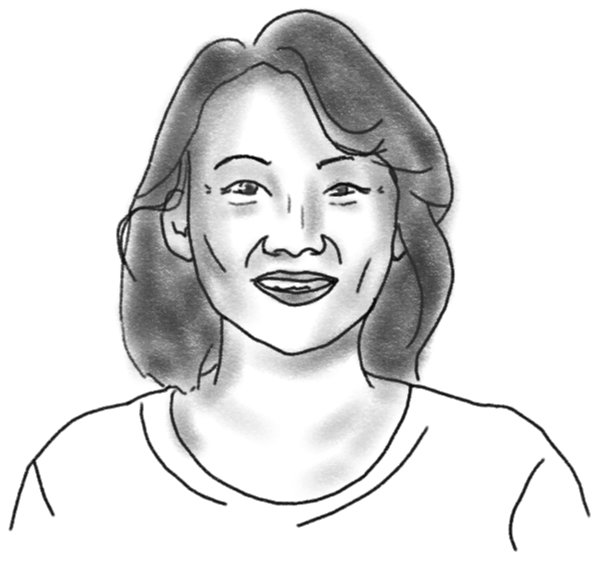
\includegraphics[width=0.9\linewidth]{portraits/hsiao-wen.png}
\end{wrapfigure}
\textbf{Hsiao-Wen Chen} is a Professor of Astronomy and Astrophysics at the University of Chicago.  She grew up in Taipei, Taiwan, and came to the US to pursue PhD in Astrophysics.  Her research interests broadly cover issues concerning the formation and evolution of galaxies across cosmic time. In particular, she is interested in studying the intricate connections between galaxies and the tenuous circumgalactic medium, in order to understand the complex physical processes that drive the gas flows in and out of galaxies.\\
\\

\vspace{-10pt}

\begin{wrapfigure}[13]{l}{0.22\textwidth}
% \vspace{-\intextsep}
\vspace{35pt}
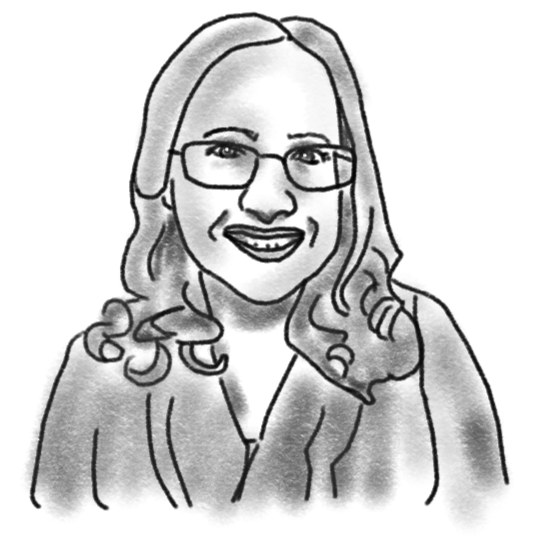
\includegraphics[width=0.9\linewidth]{portraits/deanne.png}
\end{wrapfigure}
\textbf{Deanne Coppejans} is an assistant professor of astrophysics at the University of Warwick in the United Kingdom (UK). She uses multi-wavelength observations to study the high energy astrophysics of binary stars and stellar explosions. Deanne is from South Africa. During her undergraduate studies, South Africa was competing to host the largest radio telescope on the planet (the Square Kilometre Array, SKA), and this opened her eyes to the fact that she could study the universe as a career. The South African SKA project helped her do this by funding her honours and MSc studies. With the support of the Erasmus Mundus SAPIENT programme, she then went on to do her PhD in the Netherlands. Thereafter she did a 5 year postdoc in the United States, before moving to the UK.\\
\\

\vspace{-10pt}

\begin{wrapfigure}[10]{r}{0.22\textwidth}
% \vspace{-\intextsep}
\vspace{15pt}
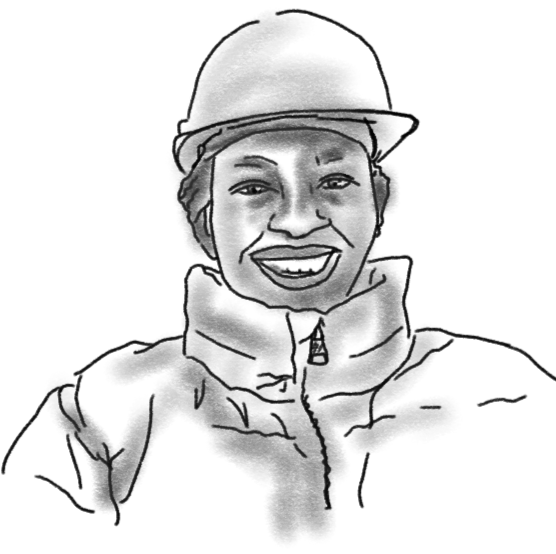
\includegraphics[width=0.9\linewidth]{portraits/sthabile.png}
\end{wrapfigure}
\textbf{Sthabile Kolwa} is obsessed with black holes and has been since first learning about them during primary school in South Africa. After completing her BSc and MSc with funding provided by the SKA project, Sthabile successfully defended her PhD thesis at the Ludwig Maximilian University of Munich in 2019. After this, she became a SARAO postdoctoral research fellow before beginning a lectureship in 2021 at the University of Johannesburg, where she now teaches physics and studies the evolution of active galaxies. Believing in the fundamental right of access to equal opportunities for all, Sthabile advocates for underrepresented groups in astronomy. \\
\\

\begin{wrapfigure}[8]{l}{0.22\textwidth}
% \vspace{-\intextsep}
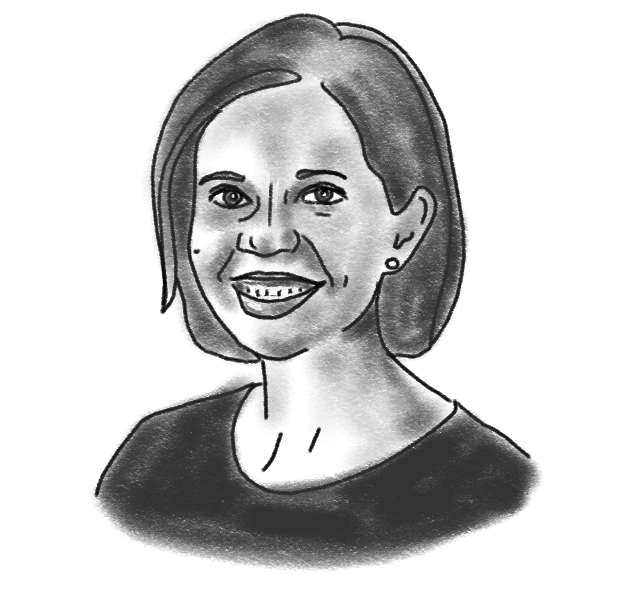
\includegraphics[width=0.9\linewidth]{portraits/raf.png}
\end{wrapfigure}
\textbf{Raffaella Margutti} grew up in a small village of $\sim4000$ people in the north of Italy and moved to Harvard as a postdoc after obtaining her PhD in Milano during which she was very fortunate to work for the Swift spacecraft. She is now an Associate Professor at UC Berkeley, where she holds a position in the Astronomy department and in the Physics department. She owes a lot to her PhD advisor Guido Chincarini who has always believed in her ideas.\\
\\

\begin{wrapfigure}[5]{r}{0.22\textwidth}
\vspace{-1.7\intextsep}
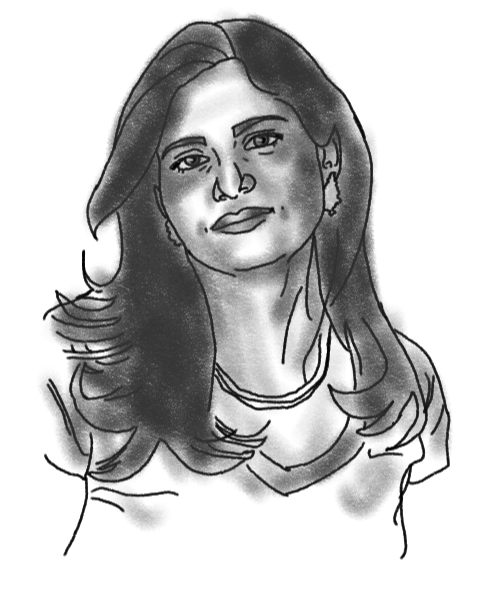
\includegraphics[width=0.9\linewidth]{portraits/priya.png}
\end{wrapfigure}
\textbf{Priyamvada Natarajan}  is a theoretical astrophysicist and is the inaugural Joseph S. and Sophia S. Fruton
Professor of Astronomy and Physics at Yale. Her research work is focused on understanding the nature of the invisible Universe, namely, black holes, dark matter and dark energy.\\
\\

% \vspace{20pt}
% \pagebreak
\begin{wrapfigure}[5]{l}{0.22\textwidth}
\vspace{-1.7\intextsep}
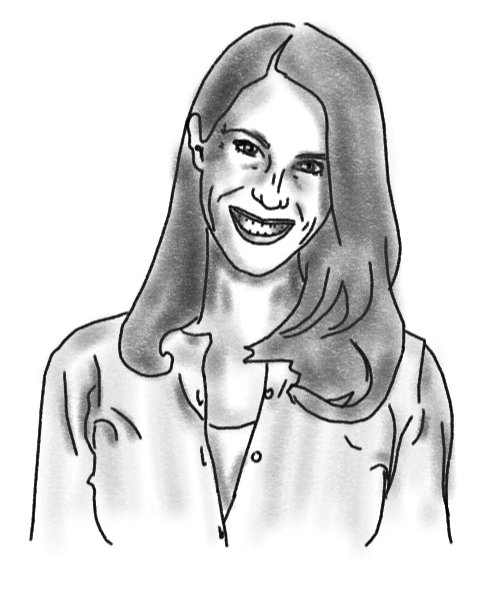
\includegraphics[width=0.9\linewidth]{portraits/erica.png}
\end{wrapfigure}
\textbf{Erica Nelson} is an astrophysicist and Assistant Professor in the Department of Astrophysical and Planetary Sciences at the University of Colorado, Boulder. She is obsessed with data on the first galaxies from the newly launched JWST and loves discovering new things about our weird and wonderful universe. \\
\\

\begin{wrapfigure}{r}{0.22\textwidth}
\vspace{-\intextsep}
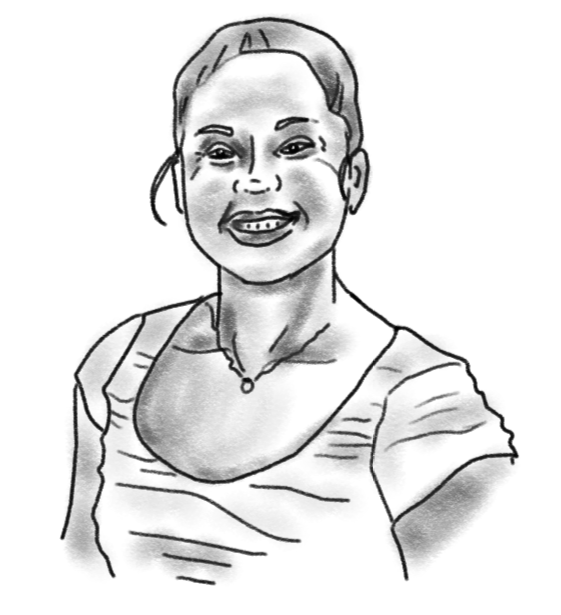
\includegraphics[width=0.9\linewidth]
{portraits/kim.png}
\end{wrapfigure}
\textbf{Kim Page} obtained both her undergraduate degree in Physics with
Astrophysics, and her PhD in X-ray Astronomy, from the University of
Leicester, UK. She has been a member of the Neil Gehrels Swift Observatory
team since before the satellite was launched in 2004, and helps to run the
UK Swift Science Data Centre based at the University of Leicester, as well
as working on X-ray observations of novae and GRBs.\\
\\

\begin{wrapfigure}[9]{l}{0.22\textwidth}
\vspace{15pt}
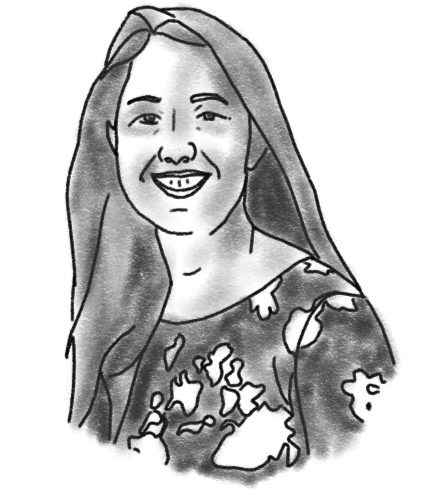
\includegraphics[width=0.9\linewidth]{portraits/silvia.png}
\end{wrapfigure}
\textbf{Silvia Toonen} is an Assistant Professor in astrophysics at the University of Amsterdam in the Netherlands. She grew up in a small town in a rural part of the country, and was the first of her family to go to university. She is interested in the ways that stars live their lives, and in particular how they interact with other stars which may lead to bright and energetic transients. Her research focuses on numerical simulations of the evolution of binary star systems, and in recent years she has pioneered the field of triple star systems.\\
\\

\begin{wrapfigure}[9]{r}{0.22\textwidth}
% \vspace{-\intextsep}
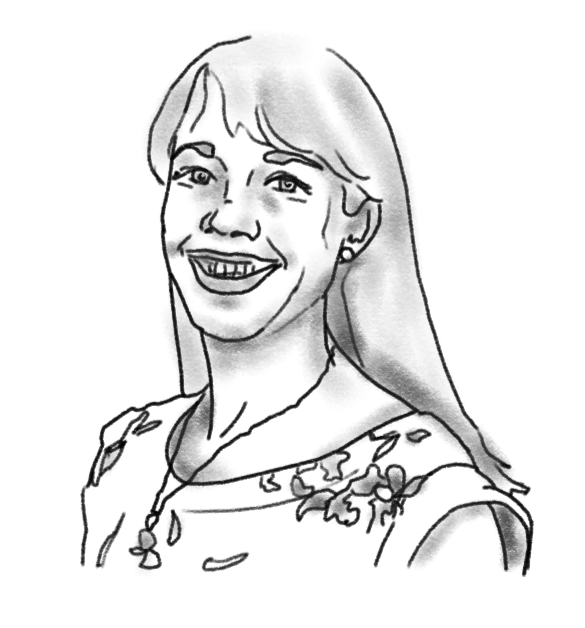
\includegraphics[width=0.9\linewidth]{portraits/katherine.png}
\end{wrapfigure}
\textbf{Katherine E. Whitaker} obtained her undergraduate degree double majoring in Physics \& Astronomy at the University of Massachusetts Amherst, and later her PhD from Yale University. She is currently an Associate Professor of Astronomy at the University of Massachusetts Amherst, as well as associate faculty at the Cosmic Dawn Center of Excellence in Copenhagen, Denmark. Her research involves understanding how the most massive galaxies evolve over billions of years of cosmic time using big telescopes in space.\\
\\

\begin{wrapfigure}[7]{l}{0.22\textwidth}
\vspace{-5pt}
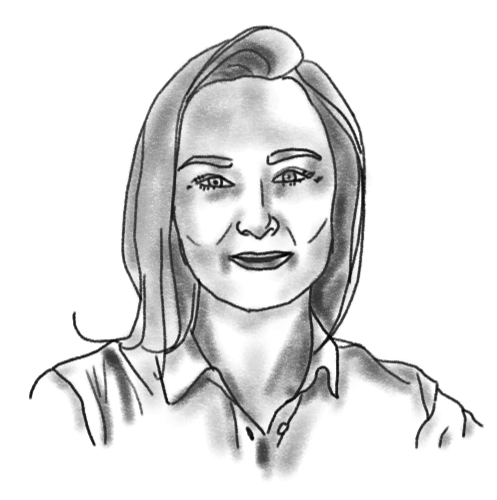
\includegraphics[width=0.9\linewidth]{portraits/irina.png}
\end{wrapfigure}
\textbf{Irina Zhuravleva} is an Assistant Professor at the University of Chicago. She is interested in the hottest and most energetic phenomena in the Universe, including interactions of supermassive black holes with galaxies and the evolution of the largest objects containing thousands of galaxies. Her studies are based on data from X-ray satellites and numerical modeling. She is also a NASA participating scientist for the recently launched XRISM satellite.